%%%%%%%%%%%%%%%%%%%%%%%%%%%%%%%%%%%%%%%%%%%%%%%%%%%%%%%%%%%%%%%%%%%%%%%%%%%
%% Ruebook RoboCup Logistics League Sponsored by Festo
%% Draft for 2013 Competition
%%%%%%%%%%%%%%%%%%%%%%%%%%%%%%%%%%%%%%%%%%%%%%%%%%%%%%%%%%%%%%%%%%%%%%%%%%%

\documentclass[12pt,twoside]{article}

\usepackage[a4paper]{anysize}
\marginsize{2.5cm}{2cm}{2cm}{2cm}

\setlength{\marginparwidth}{1cm}
\usepackage{fourier}
%\newcommand\rulechange[1]{\begin{shaded}#1\end{shaded}\marginpar{\LARGE\danger}}

%% MACROS %%%%%%%%%%%%%%%%%%%

% does not work for me, gives:
%! Undefined control sequence.
%\@ympar ...lobal \setbox \@currbox \copy \@marbox 
%                                                  \@xympar 
%\newenvironment{rulechange}{%
%  \def\FrameCommand{\fboxsep=\FrameSep \colorbox{shadecolor}}%
%  \marginpar{\vspace*{2em}\LARGE\danger} \MakeFramed  {\FrameRestore}}%
% { \endMakeFramed}
\newenvironment{rulechange}{}{}

\usepackage[load-configurations=binary]{siunitx}
% may be
%\usepackage[binary-units=true]{siunitx}
% depending on siunitx package version

%\usepackage{framed,xcolor}
%\colorlet{shadecolor}{gray!25}
\newcommand{\Robotino}{Robotino\textregistered}
\newcolumntype{R}{>{\raggedleft\arraybackslash}X}
\newcolumntype{C}{>{\centering\arraybackslash}X}

\newsavebox{\myt}
\newcommand{\mytable}[1]{\savebox{\myt}{#1}\tikz\node[fill=gray!25!white]{\usebox{\myt}};}

\newcommand{\refsec}[1]{Section~\ref{#1}}
\newcommand{\reffig}[1]{Figure~\ref{#1}}
\newcommand{\refdef}[1]{Definition~\ref{#1}}
%\newcommand{\reflst}[1]{Listing~\ref{#1}}
\newcommand{\reflst}[1]{Figure~\ref{#1}}

\usepackage{floatrow}
\newfloatcommand{capbtabbox}{table}[][\FBwidth]


%% GRAPHICSX %%%%%%%%%%%%%%%%%%%
\usepackage[pdftex]{graphicx}
\graphicspath{{figures/}}
\DeclareGraphicsExtensions{.pdf,.jpeg,.png,.JPG,.jpg}

%% TIKZ %%%%%%%%%%%%%%%%%%%
\usepackage{tikz}
\usetikzlibrary{arrows,shadows}
\usetikzlibrary{calc,positioning}
\usetikzlibrary{snakes,shapes}
\usetikzlibrary{shapes.callouts}

%% HYPERREF %%%%%%%%%%%%%%%%%%%
\usepackage{hyperref}
\hypersetup{
  pdftitle      = {The Logistics League 2013 sponsored by Festo Rulebook for 2013},
  pdfauthor     = {LLSF TC},
  pdfkeywords   = {LLSF, Rulebook},
  pdfsubject    = {},
  %pdfpagemode   = {UseOutlines},        % PageWdth, FullScreen, None ...
  hidelinks    = true,          % true colored links, false colored boxes
%  linkcolor     = black,
%  citecolor     = black,
%  filecolor     = black,
%  urlcolor      = black,
%  backref       = false,
%  pagecolor     = black,         % link to other document pages
%  linktocpage,                  % linked page numbers instead of titles
%  menucolor   = blue,           % Acrobat menu item
%  pdfnewwindow= true,                %
%  pdfborder   = {0 0 0},             %
%  bookmarksopen=true,                %
%  bookmarksnumbered=true,            %
%  pdfcreator   = {pdflatex},
%  pdfproducer  = {latex-pdftex}
}

%% SVN-MULTI %%%%%%%%%%%%%%%%%%%
\usepackage{svn-multi}

%% TODONOTES %%%%%%%%%%%%%%%%%%%
\usepackage{todonotes}

%% TIMES  %%%%%%%%%%%%%%%%%%%
\usepackage{times}

%% TABLES %%%%%%%%%%%%%%%%%%%
\usepackage{tabularx}
\usepackage{multicol}
\usepackage{multirow}
\usepackage{calc}
\usepackage{float}
\restylefloat{table}

\usepackage[TABBOTCAP]{subfigure}
%% INPUTENC %%%%%%%%%%%%%%%%%%%
\usepackage{wasysym}
\usepackage[utf8]{inputenc}
%%%%%%%%%%%%%%%%%%%%%%%%%%%%%%%%%%%%%%%%%%%%%%%%%%%%%%%%%%%%%%%%%%%%%%%%%%%%%
%%% Ruebook RoboCup Logistics League Sponsored by Festo 
%%% Draft for 2013 Competition
%%%%%%%%%%%%%%%%%%%%%%%%%%%%%%%%%%%%%%%%%%%%%%%%%%%%%%%%%%%%%%%%%%%%%%%%%%%%%


\newcommand{\s}[1]{\ensuremath{S_{#1}}}
\newcommand{\p}[1]{\ensuremath{P_{#1}}}
\newcommand{\m}[1]{\ensuremath{M_{#1}}}
\newcommand{\T}[1]{\ensuremath{T_{#1}}}
\newcommand{\dg}[1]{\ensuremath{DG_{#1}}}
\newcommand{\TAG}[1]{\texttt{#1}}



\begin{document}

%%%%%%%%%%%%%%%%%%%%%%%%%%%%%%%%%%%%%%%%%%%%%%%%%%%%%%%%%%%%%%%%%%%%%%%%%%%%%
%%% Titlepage
\pagenumbering{roman}


\begin{titlepage}
  \vspace*{5cm}
  \begin{center}
    \begin{LARGE}
      2013 Draft of the Rulebook\\[2ex]
      for the\\[2ex]
      RoboCup Logistics League sponsored by Festo\\[4ex]
    \end{LARGE}
    \hrule
    
    \vspace*{4ex}
    \begin{Large}
      The Technical Committee\\[6ex]
    \end{Large}
  \end{center}
  \vspace*{4cm}
  
  \noindent
  \svn{$Rev$}\\[2ex]
  \svn{$Author$}\\[2ex]
  \svn{$Date$}\\[2ex]  
\end{titlepage}
\thispagestyle{empty}
\pagebreak
\cleardoublepage

%%%%%%%%%%%%%%%%%%%%%%%%%%%%%%%%%%%%%%%%%%%%%%%%%%%%%%%%%%%%%%%%%%%%%%%%%%%%%
%% Table of Contents
\setcounter{page}{1}
\tableofcontents
\newpage
\cleardoublepage

%%%%%%%%%%%%%%%%%%%%%%%%%%%%%%%%%%%%%%%%%%%%%%%%%%%%%%%%%%%%%%%%%%%%%%%%%%%%%
%% 
\setcounter{page}{1}
\pagenumbering{arabic}

\todo[inline]{spell-check. American or British?}
\todo[inline]{\Robotino or Robotino throughout the doc?}

%%%%%%%%%%%%%%%%%%%%%%%%%%%%%%%%%%%%%%%%%%%%%%%%%%%%%%%%%%%%%%%%%%%%%%%%%%%%%
\section{Introduction} \label{sec:intro}

\subsection*{Preamble} \label{sec:preamble}

The future of Production Industry lies with smarter systems.  With
current developments pursuing the goal of more aware, more
decentralised behaviours in factories, a scientific platform for
applied research was required.  The RoboCup Logistics League Sponsored
by Festo (LLSF) is determined to develop into a state-of-the-art
platform for mobile robotics education. This industrial motivated
league keeps the focus on challenges promoting precise actions,
further encouraging external data supported autonomy.

This year’s competition environment is laid out in the pages to come.
It ensures the same and fair circumstances for all participants, it
however is neither meant to dictate nor suggest the way how to fulfill
the task, but is meant to develop the LLSF further towards deploying
Automated Guided Vehicles (AGV) in industrial applications. Current
challenges in developing industry-wide standards for Cyber Physical
Production Systems (CPPS) are, for instance, to design
plug-and-produce systems.

After an exciting Robocup in Mexico, we look forward to a new scale of
competition that will emerge from initiatives around the globe. In
2012 we had our first Logistics League World Champion.  In 2013 we
introduce the Referee Box changing the competition at it's core by
introducing a flow of information.  This allows for more dynamic games
and the automatic tracking of scores, and to relax the hitherto
exisiting regulations regarding additional computing power.

Finally, no rulebook is perfect. Feel obliged to inform us about
issues you like to discuss or gaps that might have an impact on the
competition, so we can keep the necessity for rule discussions at the
RoboCup event to a minimum. We are open for all kinds of suggestions;
the set of rules will be fixed at 01/01/2013 and revised in April 2013
after the German Open 2013 competition.

%%%%%%%%%%%%%%%%%%%%%%%%%%%%%%%%%%%%%%%%%%%%%%%%%%%%%%%%%%%%%%%%%%%%%%%%%%%%%
\subsection{The Task}
\label{sec:task}

Our aim is to simulate autonomous guided vehicles (AGV). In opposition
to regular automatic guided vehicles, a team, consisting of a maximum
of three Robotinos, shall complete the following task without human
interference as successful as possible competing with a second team
against the clock.

The main task is a staged production cycle of different product
variants with self-crafted intermediate products and the transport of
the final product to the delivery zone. This is the genuine goal and
will be rewarded considerably higher than partial fulfillment of the
task. The Robotinos transport hockey pucks which act as a placeholder
for (intermediate) products between the processing
machines. Basically, a machine is a signal light with an RFID reader
as described in Appendix \ref{apx:sec:engref}. If a puck is fed into
the machine, its ID tag is read and the machine reacts according to
its particular machine specification. If possible, the product is then
transformed into a new state: a new subassembly is produced. For each
product variant (cf. \refsec{sec:prodportfolio} for details), it is
required to produce the related subassemblies
step-by-step. Transformations can rely on more than one puck as input
to be triggered.

This game flow is controlled by a referee box broadcasting information
via wifi (see \refsec{sec:refbox}). It is divided into two different
phases: in an exploration phase (see \refsec{sec:expphase}) where the
Robotinos can receive scores for discovering and publishing the yet
unknown types of the different machines on the field. After this
initial phase, the referee box then announces the types of all
machines and the the second phase of the game, the actual production
task as described in detail in \refsec{sec:production-phase}, begins.

The whole factory area can be used as an intermediate
storage. Finally, the successfully assembled product has to be
delivered to the correct delivery gate and get dismounted into its
delivery slot. The factory area has to be treated in the best possible
way. Any possible damage to the field or the machines will be avenged
by the referee.

%%%%%%%%%%%%%%%%%%%%%%%%%%%%%%%%%%%%%%%%%%%%%%%%%%%%%%%%%%%%%%%%%%%%%%%%%%%%%
\subsection{Agreements \& Regulations} \label{sec:agreements}

The Logistics League follows a certain design philosophy. All teams
are obliged to use the Robotino robotic system from Festo Didactic
Gmbh \& Co. KG with certain freedoms and limitations. The usage of all
currently publicly available revisions is in order, see Section
\ref{sec:robotino} and Appendix~\ref{apx:sec:engref} for further
details.



%%%%%%%%%%%%%%%%%%%%%%%%%%%%%%%%%%%%%%%%%%%%%%%%%%%%%%%%%%%%%%%%%%%%%%%%%%%%%
%%%%%%%%%%%%%%%%%%%%%%%%%%%%%%%%%%%%%%%%%%%%%%%%%%%%%%%%%%%%%%%%%%%%%%%%%%%%%

\section{League Administration} \label{sec:commitees}
\subsection{Technical Committee 2013} \label{sec:tc}
% Alphabetical order by last name
\emph{Christian Deppe}, Otto-von-Guericke University Magdeburg, Magdeburg,
Germany\\
\emph{Daniel Ewert}, RWTH Aachen University, Aachen, Germany\\
\emph{S\"oren Jentzsch}, Technical University of Munich, Munich, Germany\\
\emph{Tim Niemueller}, RWTH Aachen University, Aachen, Germany\\
\emph{Sebastian Reuter}, RWTH Aachen University, Aachen, Germany

\medskip

\noindent
To get into contact with the TC use the mailing list\\
\centerline{\url{robocup-logistics-tc@lists.kbsg.rwth-aachen.de}.}

\subsection{Organizing Committee 2013} \label{sec:oc} \emph{Alexander
  Ferrein}, FH Aachen University of Applied Sciences,
Aachen, Germany\\
\emph{Ulrich Karras}, Festo Didactic GmbH, Denkendorf, Germany
\todo[inline]{Add missing members}

\medskip

\noindent
To get into contact with the OC use the mailing list\\
\centerline{\url{robocup-logistics-oc@lists.kbsg.rwth-aachen.de}.}


%%%%%%%%%%%%%%%%%%%%%%%%%%%%%%%%%%%%%%%%%%%%%%%%%%%%%%%%%%%%%%%%%%%%%%%%%%%%%


\section{Competition Area} \label{sec:area}


\subsection{Field dimensions} \label{sec:competition-area} The point
of origin for each statement within this rulebook that uses relative
coordinates is the bottom left corner of the competition area namely
the corner near robot insertion area below the blue input storage
area. All indicated sizes of mark-ups are to be considered outside
dimensions.

The competition area is a \SI{5.625 x 5.625}{\metre} large arena with
several RFID-mounted machines, mark-ups, a stock of raw-material and a
delivery zone. It is surrounded by boards, \SI{0.5}{\metre} of height
to reduce object interference from outside the area. The default width
for mark-ups is \SI{19}{\milli\metre}, the default color is black.

The factory area spans across \SI{4.8 x 5.625}{\metre}. There are two
boundaries, set by two mark-ups, \SI{0.4}{\metre} from the left and
right borders of the competition area. The factory area is joined by
two opposing \SI{0.4 x 1.0}{\metre} zones at the left and right
middle. The left zone is painted blue marking the \textit{input
  storage area} with the \textit{late order insertion point} to the
top. The insertion area is \SI{0.6}{\metre} of height with the
insertion slot in its middle. This spot is a \SI{0.1 x 0.1}{\metre}
empty square that will be equipped with a pallet carrier to start the
late order challenge. The space between the recycling unit and the
late order insertion point, as well as the space to the left of the
input storage area is called \textit{robot insertion area}.

The right zone is marked green and houses the three \textit{delivery
  gates}.  Each gate is of \SI{0.3}{\metre} height with
\SI{0.1}{\metre} space to the next delivery gate separated by black
mark-ups.

The delivery gates feature one signal per gate placed in middle of
each gate zone. The delivery slot resides besides a unit that is
identical in construction to a production machine. The three RFID
devices within these gates feature a black centered square of \SI{0.1
  x 0.1}{\metre} called delivery slot and residing exactly below the
RFID device. Only a pallet carrier that is delivered into the slot
completely will be considered for scoring, i.e. no part of the pallet
carrier may be outside the slot boundary.

A total of 13 machines are placed within the competition area. 10
machines representing the 3 staged production processes, 2 machines to
recycle consumed pallet carrier and 1 test station. The machines of
the production process are placed within the factory area as stated in
the table below. They are aligned in a \ang{90} angle (but which may
change during the tournament). Each production machine resides in the
centre of a squared machine space spanned by standard mark-ups with
\SI{0.6}{\metre} each side.

The 3 additional machines are arranged in the corners of the
competition area, and aligned at \ang{45}, facing the center of the
factory area. The lower left corner will remain empty. The competition
area is shown in Figure~\ref{fig:competition-area}

\begin{figure}[tb]
  \centering
  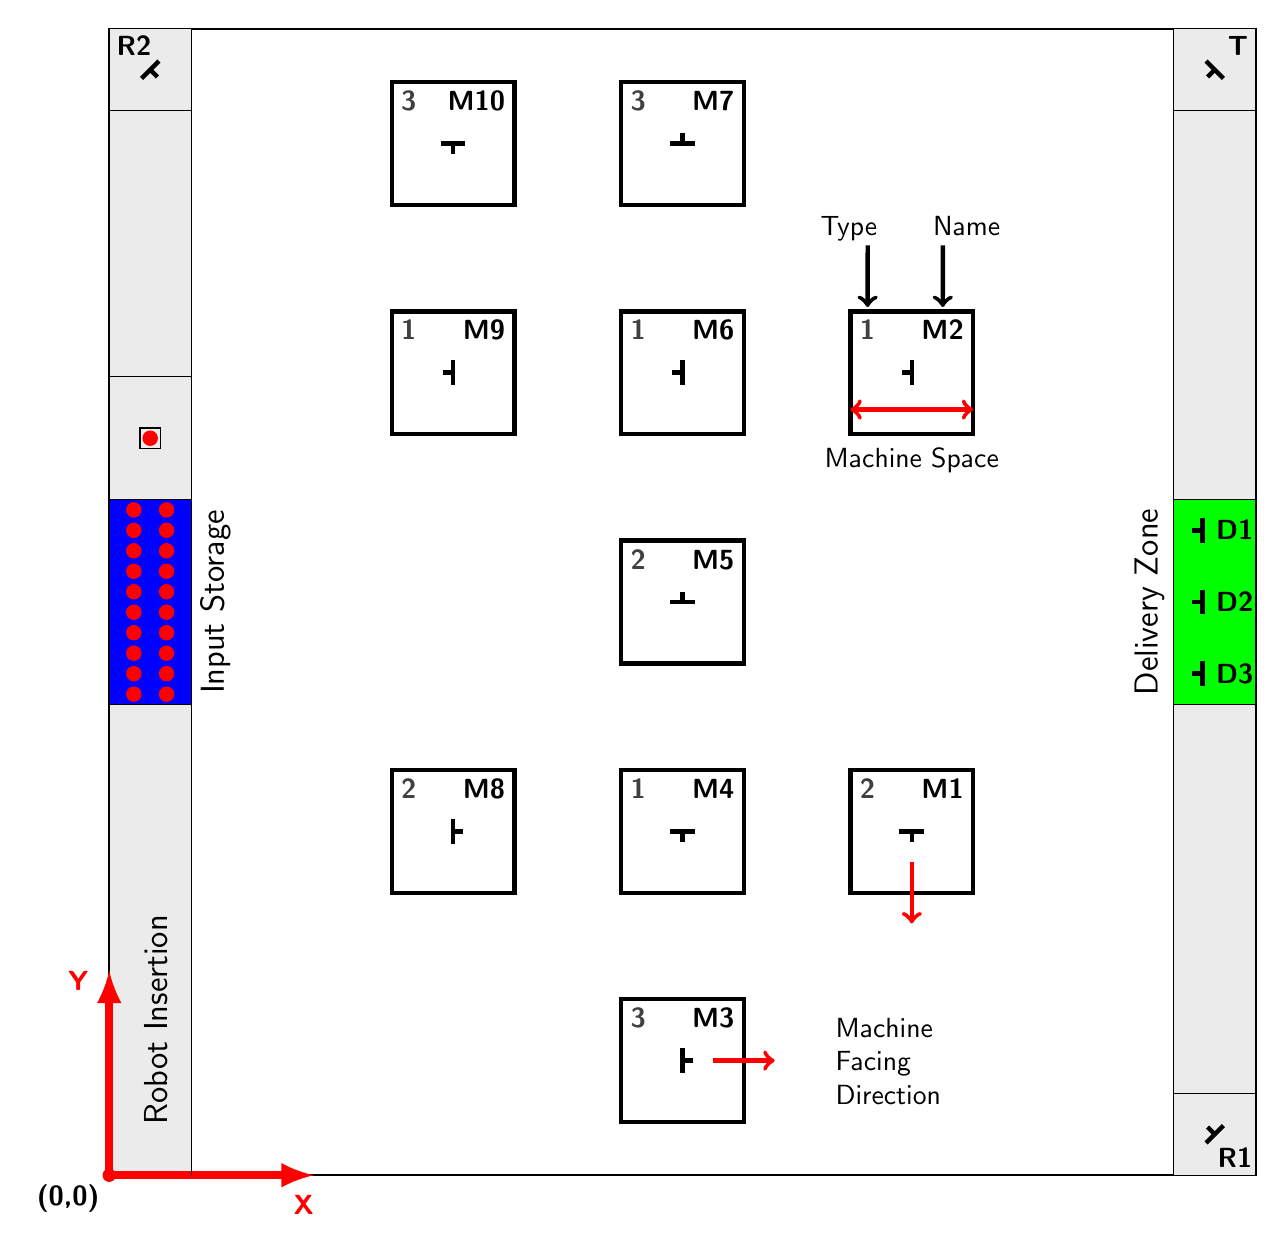
\begin{tikzpicture}[scale=2.6]
    % field outline
    \draw [thick] (0,0) rectangle (5.6,5.6);
    %\draw [fill=black!8] (0,0.4) rectangle (5.6,5.2);
    \draw [fill=black!8] (0,0) rectangle +(0.4,5.6);
    \draw [fill=black!8] (5.2,0) rectangle +(0.4,5.6);

    % coordinate system and origin
    \draw [line width=3pt,red,>=latex,->] (0,0) -- +(1,0);
    \draw [line width=3pt,red,>=latex,->] (0,0) -- +(0,1);
    \node [red,anchor=north] at (0.95,-0.05) {\sffamily\textbf{X}};
    \node [red,anchor=east] at (-0.05, 0.95) {\sffamily\textbf{Y}};
    \node [anchor=north east] at (0,0) {\sffamily\textbf{(0,0)}};
    \draw (0,0) [fill=red,draw=red] circle (0.03);

    % margin areas
    \draw (5.2,0) -- (5.2,5.6);
    \draw (0.4,0) -- (0.4,5.6);
    \draw (5.2,0.4) -- +(0.4,0);
    \draw (5.2,5.2) -- +(0.4,0);
    \draw (0,5.2) -- +(0.4,0);
    \draw (0,3.9) -- +(0.4,0); % express good area vertical line
    \draw (5.2,2.3) [fill=green] rectangle +(0.4,1);
    \draw (0,2.3) [fill=blue] rectangle +(0.4,1);
    % express good slot
    \draw (0.15,3.55) rectangle +(0.1,0.1);
    \draw (0.2,3.6) [fill=red,draw=red] circle (0.035);

    \foreach \m/\t/\x/\y/\ori/\paintbox in
    % row 1, M1 M2
    { M1/2/3.92/1.68/-90/1, M2/1/3.92/3.92/180/1,
    % row 2, M3 M4 M5
      M3/3/2.80/0.56/0/1, M4/1/2.80/1.68/-90/1, M5/2/2.80/2.80/90/1,
    % row 2, M6 M7
      M6/1/2.80/3.92/180/1, M7/3/2.80/5.04/90/1,
    % row 3, M8 M9 M10
      M8/2/1.68/1.68/0/1, M9/1/1.68/3.92/180/1, M10/3/1.68/5.04/-90/1,
    % recycling 1, recycling 2, test station
      R1/R/5.4/0.20/135/0, R2/R/0.2/5.40/-45/0, T/T/5.40/5.40/225/0,
    % delivery stations
      D1/D/5.34/3.15/180/2, D2/D/5.34/2.80/180/2, D3/D/5.34/2.45/180/2%
    }
    {
      \draw [ultra thick] (\x,\y) -- +($ (\ori-90:0.06)$);
      \draw [ultra thick] (\x,\y) -- +($ (\ori+90:0.06)$);
      \draw [ultra thick] (\x,\y) -- +(\ori:0.05);
      \if\paintbox1
        \draw [ultra thick] ($ (\x,\y) - (0.3,0.3) $) rectangle +(0.6,0.6);
        \draw [anchor=north east,inner sep=1pt] ($ (\x,\y) + (0.27,0.27) $)
          node (\m) {\selectfont\sffamily\textbf{\m}};
        \draw [anchor=north west,inner sep=1pt] ($ (\x,\y) + (-0.27,0.27) $)
          node (\m-\t) {\color{black!75}\selectfont\sffamily\textbf{\t}};
      \else
        \if\paintbox2
          \draw [anchor=west,inner sep=1pt] ($ (\x,\y) + (0.05,0) $)
            node (\m)
            {\fontsize{10pt}{10pt}\selectfont\sffamily\textbf{\m}};
        \fi
      \fi
    }

    % R and T machine descriptions
    \node [anchor=south east,inner sep=2.5pt] at (5.62,0.0) (R1)
    {\fontsize{10pt}{10pt}\selectfont\sffamily\textbf{R1}};
    \node [anchor=north west,inner sep=2.5pt] at (0,5.6) (R2)
    {\fontsize{10pt}{10pt}\selectfont\sffamily\textbf{R2}};
    \node [anchor=north east,inner sep=2.5pt] at (5.6,5.6) (R2)
    {\fontsize{10pt}{10pt}\selectfont\sffamily\textbf{T}};

    % Pucks
    \foreach \x in {1,2,...,10}
    {
      \draw ($ (0.12,2.25) + (0,\x*0.10) $) [fill=red,draw=red] circle (0.035);
      \draw ($ (0.28,2.25) + (0,\x*0.10) $) [fill=red,draw=red] circle (0.035);
    }

    \node [anchor=south west,rotate=90] at (0.33,0.2) {\large\sffamily Robot Insertion};
    \node [anchor=north,rotate=90] at (0.4,2.8) {\large\sffamily Input Storage};

    \draw [<->,red,thick,ultra thick] (3.62,3.74) -- +(0.6,0);
    \node [anchor=north] at (3.92,3.6) {\sffamily Machine Space};

    \node [anchor=south,rotate=90] at (5.2,2.8) {\large\sffamily Delivery Zone};

    \draw [->,red,ultra thick] (2.95,0.56) -- +(0.3,0);
    \draw [->,red,ultra thick] (3.92,1.53) -- +(0,-0.3);
    \node [anchor=south west,text width=1cm] at (3.5,0.3)
    {\sffamily Machine\\Facing\\Direction};

    % Name/Type explanation and arrows
    \node (name) [anchor=base west,inner sep=0pt]
    at ($ (M2.north) + (-0.05,0.4) $) {\sffamily Name};
    \node (type) [anchor=base east,inner sep=0pt]
    at ($ (M2-1.north) + (0.05,0.4) $) {\sffamily Type};

    \draw [->,black,ultra thick]
    ($ (name.base west) + (0.05,-0.05) $) -- ($ (M2.north) + (0,0.05) $);
    \draw [->,black,ultra thick]
    ($ (type.base east) + (-0.05,-0.05) $) -- ($ (M2-1.north) + (0,0.05) $);

  \end{tikzpicture}
  \caption{Competition Area}
  \label{fig:competition-area}
\end{figure}


\subsection{Coordinates of the Production Machines}
\label{sec:coordinates}

The coordinates of the machine centres and the centres of the
different field slotes are given in Table~\ref{tab:coordinates}.


\begin{figure}
\begin{floatrow}
\begin{minipage}[b]{0.5\linewidth}
  \capbtabbox{%
    \centering
    \mytable{
    \begin{tabularx}{\linewidth}{l|R|R}
      \multicolumn{1}{l}{Unit} & \multicolumn{1}{l}{$x$~[\si{\metre}]} & \multicolumn{1}{l}{$y$~[\si{\metre}]}\\ \hline
      Machine 1 & 3.92 & 1.68 \\
      Machine 2 & 3.92 & 3.92 \\
      Machine 3 & 2.80 & 0.56 \\
      Machine 4 & 2.80 & 1.68 \\
      Machine 5 & 2.80 & 2.80 \\
      Machine 6 & 2.80 & 3.92 \\
      Machine 7 & 2.80 & 5.04 \\
      Machine 8 & 1.68 & 1.68 \\
      Machine 9 & 1.68 & 3.92 \\
      Machine 10 & 1.68 & 5.04 \\
      Recycling unit 1 & 5.40 & 0.20 \\
      Recycling unit 2 & 0.20 & 5.40 \\
      Test station & 5.40 &	5.40 \\
      Late order insertion point / slot & 0.20 & 	3.60 \\
      Delivery slot 1 & 5.34 & 	3.15 \\
      Delivery slot 2 & 5.34 &	2.80 \\ 
      Delivery slot 3 & 5.34 &	2.45 \\%\hline
    \end{tabularx}  
}
      
  }{%
    \caption{Coordinates of production machines}
    \label{tab:coordinates} %
  }

  \end{minipage}
  \quad\quad
  \begin{minipage}[b]{0.2\linewidth}
  \ffigbox{%
    \centering
    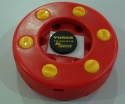
\includegraphics[width=\linewidth]{125px-Puck}    
    
  }{%
  \caption{Puck}
    \label{fig:puck}
}
\medskip\smallskip
\ffigbox{
%\begin{figure}[h]
  \centering
  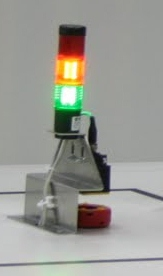
\includegraphics[width=\linewidth]{Machine}
%  \caption{Machine}
%  \label{fig:machine}
%\end{figure}

}
{  \caption{Machine}
  \label{fig:machine}
}
\end{minipage}
\end{floatrow}
\end{figure}


% \begin{table}[h]
%   \centering
%   \begin{tabular}{l|r|r}
%     \multicolumn{1}{l}{Number} & \multicolumn{1}{l}{$X~[m]$} & \multicolumn{1}{l}{$Y~[m]$}\\ \hline
%     Machine 1 & 1.68 & 1.68 \\
%     Machine 2 & 3.92 & 1.68 \\
%     Machine 3 & 0.56 & 2.80 \\
%     Machine 4 & 1.68 & 2.80 \\
%     Machine 5 & 2.80 & 2.80 \\
%     Machine 6 & 3.92 & 2.80 \\
%     Machine 7 & 5.04 & 2.80 \\
%     Machine 8 & 1.68 & 3.92 \\
%     Machine 9 & 3.92 & 3.92 \\
%     Machine 10 & 5.04 & 3.92 \\
%     Recycling unit 1 & 0.20 & 0.20 \\
%     Recycling unit 2 & 5.40 & 5.40 \\
%     Test station &	5.40  &0.20 \\
%     Late order insertion point / slot & 	3.60 & 	5.35 \\
%     Delivery slot 1 & 	3.15 & 0.26 \\
%     Delivery slot 2 &	2.80 & 0.26 \\ 
%     Delivery slot 3 &	2.45 & 0.26 \\\hline
%   \end{tabular}

%   \caption{Coordinates of production machines}
%   \label{tab:coordinates}
% \end{table}

% \begin{figure}
%   \centering
%   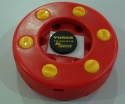
\includegraphics[height=3cm]{125px-Puck}
%   \caption{Puck}
%   \label{fig:puck}
% \end{figure}


\subsection{The Pallet Carrier Puck}
The data-carrying RFID tag is attached to top of a hockey puck. Each
pallet carrier can be identified by a unique number. The tournament puck
features a diameter of \SI{7.5}{\centi\metre} and is shown in Figure~\ref{fig:puck}.

% \begin{figure}
%   \centering
%   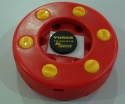
\includegraphics[height=3cm]{125px-Puck}
%   \caption{Puck}
%   \label{fig:puck}
% \end{figure}

\subsection{Machines}
\label{sec:machines}

\subsubsection{General Information}

% \begin{figure}[h]
%   \centering
%   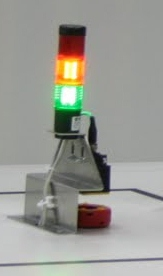
\includegraphics[height=6cm]{Machine}
%   \caption{Machine}
%   \label{fig:machine}
% \end{figure}

All machines are identical devices consisting of 
\begin{itemize}
\item one plate housing the RFID read/write device and
\item one signal unit according to Figure~\ref{fig:machine}.
\end{itemize}

They share the same design and the same RFID device, with the overall
size of (height $\times$ width $\times$ depth) \SI{280 x 160 x
  100}{\milli\metre}. Confer also Appendix~\ref{apx:sec:engref} for
  further details. The default operating mode of all machines implies
  that only the green LED is turned on. This signals that the machine
  is ready for input. The reading and writing process is a delicate
  process. To avoid corruption of the data carrier, it should not
  leave the working range of the RFID device once the processing or
  consuming is started. To enable the production process it is
  necessary to transport the pallet carrier accurately to the RFID
  device. A consumed pallet carrier has to stay within the machine
  space borders (no part of the puck being outside the mark-up) until
  the production cycle of that very machine has been
  completed. Products resulting from violating this requirement is
  considered junk and will not be rewarded. The machine always
  processes the required pallet carrier delivered last, all prior
  components will be consumed. All machines will start processing the
  data carrier as soon as it enters the machining zone as stated in
  Section~\ref{sec:competition-area} and the machine changed its
  operating mode according to 
  Tables~\ref{tab:production-machines}--\ref{tab:reading-device}.

\subsubsection{Production Machines - during exploration phase}
During the exploration pase the machines will indicate their type by individual
light signals. The light signals are defined in
Table~\ref{tab:production-machines}. Corresponding machine types will be induced
by the RefBox.

\subsubsection{Production Machines - during production phase}
After processing the current data carrier, the yellow LED is turned
on.  The machine has finished processing the current data carrier and
is waiting for the next subassembly. If the green LED is turned on,
the machine has finished the work order and is ready to receive the
next batch of carriers. In order to complete the machines' work order
the input materials have to be delivered one-by-one into the RFID
device's action range. Multiple data carriers in range of the device
will result in erroneous behaviour of the device. Consumption of
materials, such as \s0 used in the production of \s2, will take 2
seconds. Unloading the machine can be done immediately after the
operating mode changes away from processing. As long as the machines
are used properly, they will not produce any junk.

\begin{table}[tp]
\centering
\subtable[Optical Feedback during exploration phase]{\mytable{\begin{tabularx}{\linewidth}{p{0.35\linewidth}|X}\multicolumn{1}{l}{Optical Feedback} & \multicolumn{1}{l}{Operating mode} \\ \hline
  	    All LEDs turned off &  	Machine type will be induced by RefBox. \\
	    Red LED turned on &  	Machine type will be induced by RefBox. \\
        Green LED turned on &  	Machine type will be induced by RefBox. \\
        Red and Green LED turned on &  	Machine type will be induced by RefBox.\\
        All LEDs turned on  &  	Machine type will be induced by RefBox. \\
        \hline
\end{tabularx}}}

\bigskip
\subtable[Optical Feedback during production phase]{\mytable{\begin{tabularx}{\linewidth}{p{0.35\linewidth}|X}
  \multicolumn{1}{l}{Optical Feedback} & \multicolumn{1}{l}{Operating mode} \\ \hline 
  		All LEDs turned off &  	The machine is physically offline, caused by a real error which should not happen during the competition. \\
        Red LED turned on &  	The machine is out of order. \\
        Green LED turned on &  	The machine is idle and ready.\\
        Green and yellow LED turned on &  	The machine is processing or consuming the current data carrier. \\
        Yellow LED flashing (at 2 Hz) & The machine detects wrong material.
        This can be caused by data carriers that are already consumed,
        subassemblies that do not fit to this machine type's work order or
        corrupted data carriers. \\%\hline
\end{tabularx}}}

\bigskip
\subtable[Machine Types]{\mytable{  \begin{tabularx}{\linewidth}{l|X|X|X|l}
    \multicolumn{1}{l}{ Type} & \multicolumn{1}{l}{Distribution} & \multicolumn{1}{l}{Input} & \multicolumn{1}{l}{Output} & \multicolumn{1}{l}{(Final)processing time[s]}\\\hline
    \T1 & 4 times & \s0 (Raw-material) & \s1 & $t_1 = 3 \mbox{ to } 8~\mathrm{sec}$\\
    \T2 & 3 times & \s0; \s1; & \s2; one consumed container & $t_2 = 15 \mbox{ to } 25~\mathrm{sec}$\\
    \T3 & 1 times &	\s0;\s1;\s2 & \p1; two consumed containers &$t_3 = 40 \mbox{ to } 60~\mathrm{sec}$\\
    \T4 & 1 times &\s0;\s1;\s2 & \p2; two consumed containers &$t_4 = 40\mbox{ to } 60~\mathrm{sec}$\\
    \T5 & 1 times &	\s0; & \p3 &$t_5 =40\mbox{ to } 60~\mathrm{sec}$
  \end{tabularx}}}
  \caption{Production Machines}
  \label{tab:production-machines}  
\end{table}


\begin{table}[tp]
  \centering
  \mytable{\begin{tabularx}{\linewidth}{p{0.35\linewidth}|X}
    \multicolumn{1}{l}{Optical Feedback} &\multicolumn{1}{l}{Operating
      mode}\\\hline
    All LEDs turned off & 	The machine is physically offline, caused by a real error which should not happen during the competition.\\
    Red LED turned on & 	The machine is out of order\\
    Green LED turned on & 	The machine is idle and ready.\\
    Green and yellow LED turned on & The machine is processing the
    current data carrier.\\%\hline
  \end{tabularx}}
  \caption{Recycling Unit}
  \label{tab:recycling-unit}
\end{table}


\begin{table}[tp]
  \centering
  \mytable{\begin{tabularx}{\linewidth}{p{0.35\linewidth}|X}
    \multicolumn{1}{l}{Optical Feedback} &\multicolumn{1}{l}{Stored
      data on the data carrier}\\\hline
    Red LED turned on & This delivery gate is inactive.\\
    Red and green LED turned on & This gate is active, namely the designated gate.\\
%    \hline
  \end{tabularx}}
  \caption{Delivery Gates}
  \label{tab:delivery-gates}
\end{table}


\begin{table}[tp]
  \centering
  \mytable{\begin{tabularx}{\linewidth}{p{0.35\linewidth}|X}
    \multicolumn{1}{l}{Optical Feedback} &\multicolumn{1}{l}{Stored
      data on the data carrier}\\\hline
    Green LED turned on &	The station is ready to read the next data carrier.\\
    All LEDs turned off &	Consumed pallet carrier.\\
    Yellow LED turned on &	Raw-material (\s0) \\
    Red and yellow LEDs turned on & 	Subassembly 1 (\s1)\\
    Red LED turned on &	Subassembly 2 (\s2)\\
    All LEDs turned on & The final product (\p{})\\%\hline
  \end{tabularx}}
  \caption{Reading Device}
  \label{tab:reading-device}
\end{table}


The distribution describes how many machines of the respective types
will be randomly placed resulting in a the total of 10 court machines. During
th



\subsubsection{Recycling Unit (former market place)}
The recycling unit processes all supplied loading carriers back to
raw-material (\s0) within 2 seconds. The optical feedback provided by
the recycling unit differs from an ordinary production machines and is
shown in Table~\ref{tab:recycling-unit}.

\subsubsection{Delivery Gates} 

As soon as a pallet carrier is successfully delivered to the active
gate, it will show the state of the data carrier as in
Table~\ref{tab:delivery-gates}.  This state will only lasts for some
seconds and only for indicating the score to the referee. There will
be only one active gate at a time.



\subsubsection{Reading device}
Reading and visualizing the data carrier's content happens almost
instantly after delivering the pallet carrier to the action range of
the device. The optical feedback is shown in
Table~\ref{tab:reading-device}.




%%%%%%%%%%%%%%%%%%%%%%%%%%%%%%%%%%%%%%%%%%%%%%%%%%%%%%%%%%%%%%%%%%%%%%%%%%%%%
%%%

\section{The Robotino System} \label{sec:robotino}

All participants have to design their competition Robotinos within
the following specifications:

\begin{itemize}
\item Any kind of sensors can be changed or added to the Robotino
  platform.  However, it is not possible to implement sensors that
  require modifications outside the Robotino area (e.g. Northstar,
  indoor GPS).  It is furthermore strictly forbidden to implement any
  kind of RFID device into the Robotino. There must be no changes to
  the controller or mechanical system. The pushing device is defined
  as a passive, non-mechanical load handling attachment. The robots
  peripherals must neither exceed the maximum total height of
  \SI{0.7}{\metre} nor the \SI{0.4}{\metre} diameter of the body
  cylinder. The only exception to this is the one default mounted
  pushing device per robot. The pushing device can be modified; it
  however must not exceed the following outside dimensions: \SI{0.25 x
    0.15 x 0.05}{\metre}.
\item It is allowed to install additional computing power on the
  \Robotino. This may either be in form of a notebook/laptop device or
  any other computing device that suits the size requirement of the
  \Robotino{} competition system. Furthermore, it is allowed to
  communicate with an additional computing device off-field. This
  device may be used for team coordination and/or other
  purposes. However, communication among the robots and the off-field
  device is not granted during the competition.
\end{itemize}

For a detailed technical description, refer to the
Appendix~\ref{apx:sec:engref}.

\section{Communication}
Robots have to operate autonomously, that is, without any human
interference during the game. Communication among robots and to
off-board computing units is allowed only using wifi
(cf.~\refsec{sec:wifi-regulations}). Communication is not guaranteed
and maybe unavailable during parts of the game. Interruptions must be
expected and are no reason to pause or abort a game, even if they
endure for long periods of the game.

\subsection{Bandwidth Allocation}
\label{sec:bandwidth}
No minimum bandwidth is guaranteed. The amount of communicated data
over the wifi connection shall not exceed
\SI{2}{\mega\bit\per\second}. Even though the lower layers could
provide for more bandwidth, the overall available frequency spectrum
and wifi channels have to be shared, not only within our own
league. Generally, a conservative use of bandwidth resources is
advised. Should a frequently or endured exceedance of the bandwidth
limit become known, or if the overall bandwidth limit must be reduced
due to outer circumstances, the TC can monitor the network traffic and
demand reduction in communicated data as necessary.

\subsection{Referee Box}
\label{sec:refbox}
The referee box (refbox) is a software system that runs on a system
provided by the Organization Committee. It controls the overall game,
monitors feedback from team robot, and awards points. It is instructed
by an assisting human referee and keeps a log of all relevant game
events. The final game report will be produced by the refbox. While we
strive for a maximum of automation of this control task, we rely on
the human referee for final judgement, in particular for border or
underspecified cases, and will provide the largest set of override
abilities feasible.

The refbox is the single point of instruction for robots during the
game. After game setup has finished, game state information and orders
are announced by the refbox. Commands must be acknowledged. In certain
situations (for example during the exploration phase) for successful
and true communication with the refbox points are awarded. The aim is
to reduce human interference year by year to a minimum as to exhibit
the widest autonomy during the game possible. Ultimately, the refbox
should be able to fully control the game by itself, transforming all
participants, team members, and visitors alike into pure spectators of
the game, sometimes providing maintenance and crisis intervention when
necessary.

The communication from the refbox to the robot is a datagram-oriented
broadcast protocol based on Google protocol buffers\footnote{Available
  at \url{https://code.google.com/p/protobuf/}} (protobuf). The
protocol definition and technical parameters are described in detail
in the RoboCup Logistics League Referee Box Specification.

\subsection{Remote Control}
\label{sec:remote-control}
Remote operation or instruction of any kind of the robots is forbidden
at all times during a game. The only allowed interaction is for the
single button click startup (cf.~\refsec{sec:match-startup}). Any
failure to comply with this rule will lead to immediate
disqualification of the infringing team.

\subsection{Monitoring}
\label{sec:monitoring}
\emph{Passive} monitoring, i.e. receive-only communication from a base
station, of the robots' performance is allowed. However, the overall
bandwidth limit may not be exceeded.
%, this includes in particular, but
%is not limited to, images and other raw data.
If the referee has any reason to belief that a monitoring application
might be used for instruction, he can demand the shutdown of the
monitoring software (also refer to previous section on Remote
Control).

\subsection{Inter-Robot Communication}
\label{sec:inter-robot-comm}
Robots currently active on the field can freely exchange any
information that supports a coordinated team play. Robots not actively
participating in the game, for example because they have been
irrevocably removed from the current game, may not communicate with
the other robots. It is forbidden to communicate with any sensors that
are not physically attached to the robot, including, for example, but
not limited to a camera aside the field. Likewise any off-robot
actuator is forbidden.

\subsection{Communication Eavesdropping and Interference}
\label{sec:comm-tampering}
% This might sound harsh, but it's based on lessons learned in
% numerous years of RoboCup, you wouldn't believe what some teams will
% do... :-/
Communication of another team may neither be eavesdropped on nor be
interfered with. Teams not currently active shall disconnect from the
field access points.

Monitoring of bandwidth used or of possible misbehavior may only be
performed by members of the TC.
% can add this, need to be clear that this must be done using a team
% leader majority vote and not just any team leader
% or by a person appointed by the team leaders.
Any indication of misbehavior will be discussed by the team leader
convention and may result in penalties or disqualification from the
tournament.


%Each robot has to operate autonomously. The communication between the
%robot and the device responsible for the Start/Stop command, as well
%as all communication amongst the robots has to be realized using the
%Wi-Fi connection. The program controlling the robot has to be executed
%locally by the robot itself. % It is strictly forbidden to use any kind
%% of external server acting as command point.
%\begin{rulechange}
%  The robots will receive their commands from the Referee-Box as
%  specified in the referee box protocol. Further, communication to one
%  dedicated off-board computing device is allowed. However, wifi
%  communication should not taken for granted during competition by the
%  participating teams. 
%\end{rulechange}
%The robots are allowed to share information with other devices, but
%must receive nothing else but the start, pause and stop command
%from units other than the 2 fellow robots. This specifically excludes:
%Usage of processed image data created outside of the robots A central
%communication that requires a device other than the three Robotinos A
%permanently established connection between the command device and the
%Robotinos.

\subsection{Wifi regulations}
\label{sec:wifi-regulations}
In order to provide the optimal possible solution for wireless
communication during the event, all teams are required to use the \SI{5}{\giga\hertz} wifi equipment. They are furthermore required to connect their
Robotinos wifi unit to the access point provided. All teams can also
relay on wifi clients supplied by Festo but are not required to. A
detailed description concerning the infrastructure can be found in
Appendix~\ref{sec:wifi-equipment}.

% Please refer to Sect.~\ref{sec:radio-interference} for further details.

%%%%%%%%%%%%%%%%%%%%%%%%%%%%%%%%%%%%%%%%%%%%%%%%%%%%%%%%%%%%%%%%%%%%%%%%%%%%%
%%%

\section{Tournament}
\subsection{Setup}

A match is defined by two contesting teams competing at two separated
identical competition areas. Each match lasts 15 minutes with 5
minutes of setup time and a 2 minute Exploration Phase. All settings,
including the late order challenge and other random events, will be
the exact same for both parties of a match.

\subsection{Team setup}
\label{sec:team-setup}
No team member is allowed to enter the competition area prior to or
during a match. The robots can be set up within the robot insertion
area as long as they are outside the factory area and have not been
elevated into their autonomous state. During a match the manipulation
is limited to adjustments on sensors, checking cable connections and
the boot or shut down procedure. A team can ask the referee to shut
down the robot. If this motion has been forwarded within the first 15
seconds of the very robot's movement and without this robot scoring
points, the referee will move it to a point of insertion of the team's
choice, once. Otherwise or on second occasion the robot will be
removed from the competition area. Resetting or removing a robot will
not cause an interruption of the game. The referee will only interrupt
the game if there is no other way to reset the robot without
interfering with the other ongoing processes. Once removed from the
competition area the robot cannot be reinserted during the same match.
A team can also decide to remove their robot from the competition area
at any time of the match.

\subsection{Setup environment}
\subsubsection{Machine Initialization}

The physical distribution of the production machines is fixed. Their
alignment will be randomized during the event setup but will stay that
way through the whole event. The machine type of each production
machine will be randomized prior to each match. The processing time of
each machine type will be determined in the same way, so the waiting
time during a match will be static for each machine of the three
machine types (e.g. all M1 could have 7 seconds processing time). The
active delivery gate will also be randomized prior to each match but
during a match the active gate can switch.


\subsection{Game phases} \label{sec:game-phases}
\subsubsection{Exploration Phase} \label{sec:expphase} 
%
Before the actual game starts, the machines will indicate their types
with the signal lights for two minutes. The robots are to roam the
environment and announce detected signals to the referee box. Each
properly reported signal scores two points, each signal reported
wrongly will give \num{-1} points penalty. A minimum of zero points
will be accounted for this exploration phase. Production or moving
pucks is not allowed during the exploration phase.


\subsubsection{Production phase}
\label{sec:production-phase}

With the end of the exploration phase, the actual production begins,
which lasts \num{15} minutes The refbox publishes all information
regarding product and machines. All matches will start at the exact time scheduled by the organization team.
From this point on, the teams involved are allowed to start their
 robots to work autonomously within one minute. This can be done by one
 click per robot on any kind of interface. Robots which remain inactive
 after this minute will be extracted from the field.


\subsection{Production portfolio} \label{sec:prodportfolio}

The production portfolio is presented in
Table~\ref{tab:production-table} and in
Fig.~\ref{fig:production-diagram}, which presents the same information
as a production graph.



% \begin{table}[tbp]
%   \centering
%   \mytable{\begin{tabularx}{\linewidth}{c|c|c|C}
%     \multicolumn{1}{c}{Subassembly} & \multicolumn{1}{c}{Deployable} & 	\multicolumn{1}{c}{Prerequisites} & \multicolumn{1}{c}{Result}\\\hline
%     \s{0} &	\m{1}, \m{2}, \m{3}, \dg{} & 	none &	\s{1} or \TAG{consumed}\\
%     \s{1} &	\m{2}, \m{3}, \dg{} &  	\s{0} & 	\s{2} or \TAG{consumed}\\
%     \s{2} & \m{3}, \dg & 	\s{0}, \s{1} &	\p{}\\ %
%     \TAG{Late Order} &  	\m{1} & none &  \TAG{Finished Late Order}\\
%     \hline
%   \end{tabularx} }
%   \caption{The production table}
%   \label{tab:production-table}
% \end{table}


% \begin{figure}[tbhp]
%   \centering

% \tikzstyle{M}=[rectangle, draw=blue, thick, fill=blue!20, text width=2em,align=center, rounded corners, 
%   minimum height=2em]
% %
% \tikzstyle{P}=[draw=red, thick, circle,fill=red!20, minimum height=1.5em]

% \begin{tikzpicture}[level distance=4em,sibling distance=5em]
%   \node[P] {$S_1$}  [grow=left,thick]
%   child { node[M] {$M_1$}
%     child { node[P] {$S_0$}}};
% \end{tikzpicture}
% \hspace*{1em}
% \begin{tikzpicture}[level distance=4em,sibling distance=5em]
%   \node[P] {$C$}  [grow=left,thick]
%   child { node[M] {$M_1$}
%     child { node[P] {$S_0$}}};
% \end{tikzpicture}

% \begin{tikzpicture}[level distance=4em,sibling distance=5em]
%   \node[P] {$C$}  [grow=left,thick]
%   child { node[M] {$M_2$}
%     child { node[P] {$S_0$}}
%     child { node[P] {$S_1$}}
%     child { node[P] {$S_2$}}
%     };
% \end{tikzpicture}

% \begin{tikzpicture}[node distance=4em,level distance=4em,sibling distance=5em]

%   \node[P] (p) {$P$}  [grow=left,thick]
%   child { node[M] (m) {$M_3$}
%     child { node[P] {$S_0$}}
%     child { node[P] {$S_1$}}
%     child { node[P] {$S_2$}}
%    };
  
% \end{tikzpicture}


%   \caption{The production diagram}
% \label{fig:production-diagram}  
% \end{figure}





\begin{figure}
\begin{floatrow}
  \capbtabbox{%
    \centering
    \mytable{\begin{tabularx}{\textwidth}{C|C|C|c}
        \multicolumn{1}{c}{Subassembly} & \multicolumn{1}{c}{Deployable} & \multicolumn{1}{c}{Prerequisites} & \multicolumn{1}{c}{Result}\\\hline
        \s{0} &	\T{1}, \T{2}, \T{3}, \T{4}, \T{5} & none & \s{1}, \p{3} or
        \TAG{consumed}\\
        \s{1} &	\T{2}, \T{3}, \T{4} &  	\s{0} & 	\s{2} or \TAG{consumed} \\
        \s{2} & \T{3}, \T{4} & \s{0}, \s{1} &	\p{1}, \p{2} \\
        \TAG{Late Order} & \T{1} & none &  \TAG{Finished Late Order}\\
%        \hline
      \end{tabularx}
    }      
  }{%
    \caption{The production table}
    \label{tab:production-table}
  }
\end{floatrow}
  
\bigskip
\begin{floatrow}
  \ffigbox{%
    \centering
    
    \tikzstyle{M}=[rectangle, draw=blue, thick, fill=blue!20, text width=2em,align=center, rounded corners, 
    minimum height=2em]
    % 
    \tikzstyle{P}=[draw=red, thick, circle,fill=red!20, minimum height=1.5em]
    
\begin{tikzpicture}[level distance=4em,sibling distance=5em]
  \node[P] {$S_1$}  [grow=left,thick]
  child { node[M] {$T_1$}
    child { node[P] {$S_0$}}};
\end{tikzpicture}

\bigskip
\bigskip

\begin{tikzpicture}[level distance=4em,sibling distance=5em]
  \node[P] {$S_2$}  [grow=left,thick]
  child { node[M] {$T_2$}
    child { node[P] {$S_0$}}
    child { node[P] {$S_1$}}
    };
\end{tikzpicture}


\bigskip
\bigskip

\begin{tikzpicture}[node distance=4em,level distance=4em,sibling distance=5em]
  \node[P] (p) {$P_1$}  [grow=left,thick]
  child { node[M] (m) {$T_3$}
    child { node[P] {$S_0$}}
    child { node[P] {$S_1$}}
    child { node[P] {$S_2$}}
   };  
\end{tikzpicture}
\bigskip
\bigskip

\begin{tikzpicture}[node distance=4em,level distance=4em,sibling distance=5em]
  \node[P] (p) {$P_2$}  [grow=left,thick]
  child { node[M] (m) {$T_4$}
    child { node[P] {$S_0$}}
    child { node[P] {$S_1$}}
    child { node[P] {$S_2$}}
   };  
\end{tikzpicture}

\bigskip
\bigskip

\begin{tikzpicture}[level distance=4em,sibling distance=5em]
  \node[P] {$P_3$}  [grow=left,thick]
  child { node[M] {$T_5$}
    child { node[P] {$S_0$}}};
\end{tikzpicture}

}{%
  \caption{The production diagram}
  \label{fig:production-diagram}  
}
\end{floatrow}
%\todo[inline]{What is a C??}

\bigskip
\begin{floatrow}
  \capbtabbox{%
    \centering
    \mytable{\begin{tabularx}{0.75\textwidth}{X|X}%{p{0.35\textwidth}|p{0.65\textwidth}}
        \multicolumn{1}{l}{Product variant} &\multicolumn{1}{l}{Demanded number of items } \\
        \hline 
        Product variant \p1 &	$N_1 = 1 \mbox{ to } 10$ items \\
        Product variant \p2 &	$N_2 = 1 \mbox{ to } 10$ items \\
        Product variant \p3 &	$N_3 = 1 \mbox{ to } 10$ items \\
        %	\hline
      \end{tabularx}}
  }{
    \caption{Production plan}
    \label{tab:production-plan}
  }
\end{floatrow}
\end{figure}






% \newcommand{\varone} {
%   \begin{tikzpicture}[level distance=4em,sibling distance=5em]
%     \node[P] {$P$}  [grow=left,thick]
%     child {node[M] {$M_3$} 
%       child {node[P] {$S_0$}} 
%       child {node[P] {$S_1$}
%         child {node[M] {$M_1$} 
%           child {node[P] {$S_0$}}
%         }
%       } 
%       child {node[P, yshift=-1em] {$S_2$}
%         child {node[M] {$M_2$} 
%           child {node[P] {$S_0$}}
%           child {node[P] {$S_1$}
%             child {node[M] {$M_1$}
%               child {node[P] {$S_0$}}
%             }
%           }
%         }
%       }
%     };
%   \end{tikzpicture}
% }

% \newcommand{\varthree} {
%   \begin{tikzpicture}[level distance=4em,sibling distance=5em]
%     \node[P] {$P_2$}  [grow=left,thick]
%     child {node[M] {$M_3$} 
%       child {node[P] {$S_0$}}
%       child {node[P] {$S_2$}}
%       child {node[P] {$S_2$}}      
%     };
%     \end{tikzpicture}
% }

% \newcommand{\vartwo} {
%   \begin{tikzpicture}[level distance=4em,sibling distance=4em]
%     \node[P] {$P$}  [grow=left,thick]
%     child {node[M] {$M_3$} 
%       child {node[P] {$S_0$}}
%       child {node[P] {$S_1$}}
%       child {node[P,label={[label distance=-6pt,fill=red!20]270:{\footnotesize $0.5$}}] {$S_2$}}
%       child {node[P,label={[label distance=-6pt,fill=red!20]270:{\footnotesize $0.5$}}] {$S_2$}}      
%     };
%     \end{tikzpicture}
% }


% \begin{tikzpicture}
%   \matrix[anchor=east]{
%     \node (p1) {\varone};\\
%     \node (p2) {\vartwo};\\[2ex]
%     \node (p3) {\varthree};\\
%   };
% \end{tikzpicture}


\subsubsection{The production table}

Table~\ref{tab:production-table} shows the production table for the
main challenge; the three staged production process as well as the
Late Order challenge. The main challenge can be repeated as long as
enough pallet carriers can be provided to complete the cycle. The
different machine types are specified in Sect.~\ref{sec:machines}.



\subsubsection{Late order}

The late order challenge will be announced by the referee box. The
challenge requires a fast paced processing and delivery of the
requested product within a specified time window. The challenge also
requires prior knowledge concerning the machine distribution.

\subsection{During a match}

Any referee can interrupt the match at any time. After the referee box
is stopped, both teams have 5 seconds to stop all robot movement. The
match time will be paused during the interruption. A team can decide to
stop the autonomy process of each robot individually at any time of the
match. Doing so has to be announced notably in order to inform the
referee, as this is considered a shut down request according to
\ref{sec:team-setup}. Robots that do not stop within the time limit
will be treated in the same way. Any robot can only be stopped one
time. A second stop announcement leads to permanent extraction of the
related robot.

\subsubsection{Out-of-order}

The downtime generator will take down a maximum of two machines out of
the pool containing production machines and recycling units. It will
do so at random points of time. There will be 6 to 8 of such triggered
events during a match. The machines affected will remain out of order
for 60 to 120 seconds. Every machine can only be forced out of order
once per match. If the machine turns offline during processing or
consumption of mounted a pallet carrier, it will afterwards resume the
process.

\subsubsection{Production Plan}

The referee box will announce a production plan for different
phases of the match. The production plan specifies how many items of
different product variant have to be produced in the current production phase.
The number of items can range from 1 to 10 items per phase. Only products which
are covered by the production plan score. In 2013 there will be three phases.
Each of the three phases will last 5 minutes. The first phase will start with
the match startup. The second phase will start at minute 5, the third at minute
10. The production plan is shown in Table~\ref{tab:production-plan}.

% \begin{table}[t]
%   \centering
%   \mytable{\begin{tabularx}{\linewidth}{p{0.35\linewidth}|X}
%     \multicolumn{1}{l}{Product variant} &\multicolumn{1}{l}{Demanded number of items } \\
%     \hline 
%     Product variant \p1 &	$N_1 = 1 \mbox{ to } 10$ items \\
%     Product variant \p2 &	$N_2 = 1 \mbox{ to } 10$ items \\
%     Product variant \p3 &	$N_3 = 1 \mbox{ to } 10$ items \\
%     %	\hline
%   \end{tabularx}}
%   \caption{Production plan}
%   \label{tab:production-plan}
% \end{table}

\subsubsection{Late order challenge}

The challenge will be induced by the referee box sending an late order
message to the robots. The message specifies the demanded product
variant, a time window and the delivery gate. As a first step, the late
order challenge of 2013 will only demand for product variant
\p3. Furthermore, in 2013 the challenge has to be completed within a
time window of 120 seconds and the late order has to be delivered to
the active delivery gate. 

\subsection{Mode}
\subsubsection{Tournament scoring specifications}

% The tournament features two stages with the first stage being done in
% league form with several sequels orientating at the number of
% participants and a second stage with playoffs featuring the top 4
% teams.

\paragraph{Round-Robin phase} 
There will be two stages in the competition. The first stage is a
group phase and will be played as a round-robin. The best 4 teams of
the round-robin stage will advange to a playoff round.
%
At the round-robin stage, the teams will be receive the true point
they scored by delivering and producing goods during the
competition. The points will be accumulated in this phase and the
teams will be ranked according to the accumulated point in descending
order.

\paragraph{Playoffs} At the payoff stage, the scoring scheme will be
different. As each team in this phase directly competes with an
opposing team, the team that scores more points as the direct
opponent, will be announced as the winner and 3 points will be awarded
to this team. A loss will be awarded with 0 points. Additionally, if
both teams are unable to score any points during the match by
delivering or producing goods, both team will receive 0 points.
%
% Each match will be resulted with the score of each team. The winning
% team will be awarded 2 major points. In case of a draw both teams will
% be awarded with 1 major point. In case both teams scored zero points,
% no major points will be awarded.
%
In case of a draw within the playoffs, the game time will be extended
by 5 minutes unless both teams scored zero points.
%
If this extension leads to a draw too the overall regular points of
the teams will determine the match winner. If the overall points are
equal too, a direct comparison between the teams in question will
decide. If this fails to resolve the situation, the teams will
approach a coin toss to determine the winner.



\paragraph{Finals.} The best 2 teams of the playoff phase will advance
to the finals. The competition mode for the final is the same as in
the playoff phase.

\bigskip
The detailed seeding will be created at the event. Although the idea
is to allow each participant to challenge each other team the league
can be adjusted to meet time requirements.


\subsubsection{Tournament challenge}
Proceeding to the playoffs will result in the following changes to the
late order challenge setup:
% \begin{table}[h]
%   \centering
%   \begin{tabularx}{\linewidth}{l|X}
%     \multicolumn{1}{l}{Phase} &\multicolumn{1}{l}{Remark}\\\hline
%     \multirow{7}{*}{League phase} & 
%     \begin{itemize}\itemsep-3pt
%     \item The active delivery gate will not switch during a match.
%       % 
%     \item There will be 3 express good challenges.
%       % 
%     \item     No challenge will be initialised during the first or within the last two match minutes.
%     \end{itemize} \\
%     \multirow{9}{*}{Playoffs} &
%     \begin{itemize}\itemsep-3pt
%     \item The active delivery gate will swap twice - after minutes 7
%       and 11. A delivery made to the old active gate will be still
%       valid for the next 10 seconds.
%       % 
%     \item There will be 4 express good challenges. 
%       % 
%     \item No challenge will be initialised during the first or within
%       the last two match minutes.
%     \end{itemize}\\\hline
%   \end{tabularx} 
%   \caption{Tournament Phases}
%   \label{tab:phases}
% \end{table}

\paragraph{League phase}
\begin{itemize}
\item The active delivery gate will not switch during a match.
\item There will be 3 late order challenges.
\item No challenge will be initialised during the first or within the
  last two match minutes.
\end{itemize} 


\paragraph{Playoffs}
\begin{itemize}
\item The active delivery gate will swap twice - after minutes 7
  and 11. A delivery made to the old active gate will be still
  valid for the next 10 seconds.
\item There will be 4 late order challenges. 
\item No challenge will be initialised during the first or within
  the last two match minutes.
\end{itemize}    


In both cases, delivered or timed out pallet carriers will be removed
from the game by the administration and therefore cannot be recycled.



\begin{table}[tb]
  \centering
  \subtable[Scoring scheme for the main challenge]{\mytable{\begin{tabularx}{\linewidth}{p{6em}|X|p{4em}}
      \multicolumn{1}{l}{Subtask } &\multicolumn{1}{l}{Main challenge} &
      \multicolumn{1}{l}{Scoring [Point]}\\\hline
      Produce \s2 & Finish the work order of a machine type 2 & $+4$\\
      Produce \p  & Finish the work order of a machine type 3 & $+12$ \\
      Deliver & Deliver the final product to the designated loading zone & $+5$\\
      Recycle & Clean up a polluted machine (\m2 or \m3) by recycling all
      of the 3 consumed loading carriers. Partial recycling(\m3) will not
      be rewarded.&
      \multirow{3}{*}{$\begin{array}{l}+3 - \m2\\
          +6 - \m3\end{array}$}\\
      Sum &Total points a team will receive for a produced and correctly
      delivered final product with its consumed loading carrier
      recycled. & $30$\\%\hline
    \end{tabularx}  }}


  \bigskip
  \subtable[Scoring scheme for the Late order challenge]{\mytable{\begin{tabularx}{\linewidth}{p{6em}|X|p{4em}}
    \multicolumn{1}{l}{Subtask } &\multicolumn{1}{l}{LOC - Late Order
      Challenge} & \multicolumn{1}{l}{Scoring [Point]}\\\hline
    Finish the EG &	Deliver the EG to a machine of type 1 and process the late order in time if the machine type was identified by an earlier production process. &	+5\\
    Deliver the EG & Deliver the processed the late order to the active
    delivery gate in time. &  +10\\
    Sum & In time delivery of a correct late order. & 15\\%\hline
  \end{tabularx} }}
  \caption{Scoring Scheme}
  \label{tab:scoring}   
\end{table}


\subsubsection{Task fulfilment}

Table \ref{tab:scoring} provides the itemized clearance of all task
related processes.




\subsection{Penalties}

The catalogue in Table~\ref{tab:infringements} represents the decision
basis for the referees without being exhaustive or binding.
%
The abidance of these rules will be monitored by at least two
referees.  One ``field'' referee will overlook the competition
area. The field refereee is allowed to enter the area at any
time. Accidental moving of a puck or similar unintended tampering
resulting from the referees present on the field must be coped with. A
second "station" referee operates the control station for the refbox
to issue the initial start command and monitor the game flow and the
correctness of the digital representation and automatical scoring.


\begin{table}[th]
  \centering
  \mytable{
    \begin{tabularx}{\linewidth}{l|X}
  \multicolumn{1}{l}{Issue} &\multicolumn{1}{l}{Sanction}\\\hline
  Premature movement & No robot is allowed to move until the referee
  announced the start of the match The faulty robot will be grounded
  for
  2 minutes\\[1ex]
%
  Damaging factory equipment & Theoretical damage to the real
  factory equipment as a result of collisions and negligent actions.
  This behaviour will be punished as a minor rule break.\\[1ex]
  % The team will be punished with a score reduction. The total score
  % cannot  drop below zero.\\[1ex]
%
  Not showing up & A team not showing up at all. The team will be
  removed from the tournament unless the team leader can provide a
  sincere explanation.\\[1ex]
%
  Manual Interference & A manual interference of a team, i.e. touching
  a robot without the referee's permission, during the game will be
  punished as a major rule break.\\[1ex]
%
  Breaking a minor rule & A rule infringement with minor impact on the
  team performance or competition mechanics. Upon decision of
  the referee, 25 \% of the scored points of the team at the time of
  the infringement will be deducted, at least 1 point.\\[1ex]
  %
  Breaking a major rule & A rule infringement with considerable impact
  on the team performance or competition mechanics. Upon decision of
  the referee, 50 \% of the scored points of the team at the time of
  the infringement will be deducted, at least 5 points. \\[1ex]
  % The referee will
  % decide upon calling a team vote or imposing an adequate punishment.\\[1ex]
  % 
  Arguing with the referee & There will be no discussions during a
  match. Each team can make a motion to protest a certain match and
  its result which will be dealt with after the match. There will be a
  warning. Continued disregard will result in a time punishment to the
  team's current or next match.\\[1ex]
%
  Disregarding rules of conduct & Following the rules of conduct
  should be self-explanatory Upon disregard, the referee will impose
  sanctions ranged from time punishments to the team's complete
  removal from the tournament.\\%\hline
  \end{tabularx}  }
  \caption{Infringements}
  \label{tab:infringements}
    
\end{table}


  \subsection{Technical Challenge}
  
  Within the league, the technical advances should be documented from
  year to year. Therefore, the Technical Challenge is introduced.
  Each participating team should prepare for participating in any
  number the following tasks:


  \paragraph{Collision avoidance.~}
  The robot is to show that it avoids other obstacles and robots.
  Therefore the robot must drive from the input storage to the delivery zone.
  However, the paths between the input storage and the delivery zone will
  be blocked randomly by static obstacles and the robot must not touch any
  of the obstacles. For touching an obstacle, the team receives a penalty.
  The fastest team with the fewest penalty points to reach the delivery
  zone wins this challenge. All other teams are ranked according to
  how fast they were and how many penalties they conceived.
  
  \paragraph{Whac-a-Mole.~}
  A single robot is placed somewhere on the field. It has to detect
  the single shining signal unit on the play field. As soon as it puts
  a puck underneath it, the signal unit is switched off and another
  random signal unit is switched on. The goal of the challenge is to
  switch as many signal units as possible within a given time
  frame. Teams are ranked according to the number of turned-off
  signals.
  

  \paragraph{Free challenge.~}
  Each team will be given 5 minutes to showcase their robot team, e.g.
  show some new robotics developments. The team leaders of
  non-presenting team will judge the performance and rate it with
  points between 0--10.  The team with the most points will win this
  challenge. The other teams are ranked in decreasing point order.


  The technical challenge is conducted in the following way: The
  team leader of each participating team agree on a date and time
  during the tournament for the Technical Challenge in their first
  Team leader Meeting. Each team can register for any of the
  challenges. All team leaders have to be present at the time of the
  challenge to judge the other teams. The OC is responsible to conduct
  the Technical Challenge and can appoint team leaders to support in
  conducting the challenges. Each challenge will have a separate
  ranking. In each ranking, the team on the last rank will receive 0
  points, the last-but-one ranked team will receive 1 point etc. The
  points for each ranking will be added and the team with the most
  points accrued over all challenges will be awarded with the
  LLSF Technical Challenge Award.




%%%%%%%%%%%%%%%%%%%%%%%%%%%%%%%%%%%%%%%%%%%%%%%%%%%%%%%%%%%%%%%%%%%%%%%%%%%%%
%%%

% \section{Development / Vision}

% This section is meant to enable discussions and support investment
% decisions for future soft- and hardware acquisitions.

% \subsection{Short term ideas}

% These are ideas that could still be incorporated into the rulebook of
% Istanbul 2011. 

% \subsubsection{Scripted, dynamic obstacles}

% On the way to fully dynamic obstacles this iteration implies a fully
% scripted administration controlled Robotino that follows implicit
% movement rules that are known to all participants.

% \subsection{Midterm planning}
% Additions and alterations for future iterations of this competition


% \subsubsection{Various Production programs}
% A part from the three-staged production process, various goods with
% different work orders and specifications (e.g. top speed, delivery
% strategies...) could be part of the challenge. This addition seems to
% be heavily dependent on Sect.~\ref{sec:supp-flow}.

% \subsubsection{Various order strategies}
% A delivery could consist of more than one final product, it could be
% required to deliver a batch of products, maybe within a certain time
% span, to complete the loading and receive extra points. Also, the
% different delivery gates could obtain a predefined shipping list, for
% example gate 1 requiring 2 Products, 2 M2 and 1 M1, maybe in the
% correct order to enable FIFO, LIFO or other delivery strategies.

% \subsubsection{Simulation league}

% Since there is only the annually world championship and maybe a
% regional preregistration, a simulation platform could be provided,
% where the software framework of teams can be used to compete with
% other teams. Additionally a branch of simulation could be created that
% focuses on the simulation of many AGV and a huge production area in
% order to compete on scalability.

% \subsubsection{Introducing a supportive flow of information}
% \label{sec:supp-flow}

% As the current task only deals with the material stream, it is heavily
% limited to a simple static task. In order to enable a flow of
% information that transports complex orders, a combined effort should
% focus on implementing a data interface that can be used by all teams
% today and in the future. As this would be a giant leap towards the
% industrial application, a general discussion and a lot of effort has
% to be invested into this issue.


% \subsection{Long term Vision}
% Ideas, dreams and ideology that inspire the future development.

% \subsubsection{Complex production machines}
% As there are more ways to interact with a machine than mounting and
% dismounting a loading carrier, it is possible to develop new machine
% types that look different and are completely different to handle.

% \subsubsection{Collaborative Production}
% Teams could be required to cooperate with another team to enable a
% combined supply chain. 

% \subsubsection{Opponent controlled dynamic obstacles}
% No scripted obstacle can truly represent challenges of the industrial
% application. In the long run, an opposing team has to be reinserted
% that is allowed and requested to anticipate the logistic processes in
% real time in order to create worst case scenarios for the teams.

% \subsubsection{Interfacing ERP / SCM}
% The interface used to present orders could be back ended with software
% from real business applications like ERP, PPS, WHM and SCM.

% \subsubsection{JIS / JIT implementation}
% With complex production processes and several other achievements and
% upgrades it could be useful to implement JIS and JIT tasks and
% procedures into the LL, requiring delivery strategies like LIFO, FIFO
% and certain time windows.

%%%%%%%%%%%%%%%%%%%%%%%%%%%%%%%%%%%%%%%%%%%%%%%%%%%%%%%%%%%%%%%%%%%%%%%
%%% 

\begin{appendix}
\newpage

\section{Engineering reference} \label{apx:sec:engref}
\subsection{The Mobile Robot System}
The mobile robot system Robotino® is a platform with an open
mechanical interface for the integration of additional mechanical
devices and an open electrical interface to integrate easily
additional sensors or motors of devices. Power is supplied via two
\SI{12}{\volt} lead gel batteries which permit a running time of up to
two hours.  The scope of delivery likewise includes a charging
device. Robotino® is driven by 3 independent, omnidirectional drive
units. They are mounted at an angle of \ang{120} to each other. The
three omnidirectional drive units of Robotino® , defines the robot as
being holonomic, meaning that the controllable degrees of freedom
equals the total degrees of freedom of the robot. The drive units are
integrated in a sturdy, laser welded steel chassis. The chassis is
protected by a rubber bumper with integrated switching sensor.

\subsubsection{Robot dimensions}
\begin{itemize}
	\item[] \textbf{Diameter:} \SI{370}{\milli\metre}
	\item[] \textbf{Height including housing:} \SI{210}{\milli\metre}
 	\item[] \textbf{Overall weight:} approx. \SI{11}{\kilogram}
 	\item[] \textbf{Maximal payload:} about \SI{6}{\kilogram}
 \end{itemize}

\subsubsection{Drive Unit}
Each of the 3 drive units consists of the following components: DC
Dunker motor with nominal speed of \SI{3600}{rpm} and nominal torque
of \SI{3.8}{\newton\centi\metre}. Integrated planetary gear unit with
a gear ratio of 4:1. Omnidirectional wheels of diameter of
\SI{80}{\milli\metre}. Toothed belt with gear wheels providing a
transmission ratio of 4:1.
%
Altogether this provides a gear transmission ratio of
16:1. Incremental encoder with a resolution of 2048 increments per
motor rotation.
%
The motor and gear arrangement is shown in
Figure~\ref{apx:fig:driveunit}.

\begin{figure}[tbh]
\centering
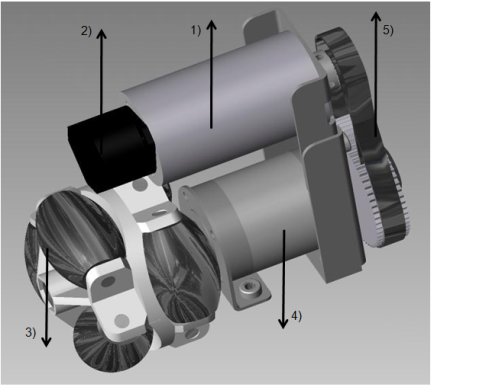
\includegraphics{driveunit.png}
\caption{Drive unit with motor (1), encoder (2), omnidirectional wheel
(3)}
\label{apx:fig:driveunit}
\end{figure}

The motor speed will be controlled via a PID controller implemented on
a Atmel microprocessor of the controller board of Robotino®.

\subsubsection{Sensors}

Robotino® is equipped with 9 infrared distance measuring sensors which
are mounted in the chassis at an angle of \ang{40} to one
another. Robotino® can scrutinise all surrounding areas for objects
with these sensors.  Each of the sensors can be queried individually
via the controller board. Obstacles can thus be avoided, clearances
can be maintained and bearings can be taken on a selected target. The
sensors are capable of accurate or relative distance measurements to
objects at distances of \SI{4}{\centi\metre} to
\SI{30}{\centi\metre}. Sensor connection is especially simple
including just one analogue output signal and supply power. The
sensors’ evaluation electronics determines distance and read it out as
an analogue signal.  The anti-collision sensor is comprised of a
switching strip which is secured around the entire circumference of
the chassis. A reliably recognisable signal is thus transmitted to the
controller unit.  Collisions with objects at any point on the housing
are detected and, for example, Robotino® is brought to a
standstill. The inductive proximity sensor is supplied as an
additional component. It serves to detect metallic objects on the
floor and is used for continuous-path control, e.g. it might be used
to detect the blue lines (metallic stripes) on hockey field. It reads
out signals of varying strength depending upon whether it is located
in the middle or at the edge of the metal strip. Path tracking can
thus be controlled in a differentiated fashion.

The inductive proximity sensor must be attached to the mounting
furnished for this purpose, and must be connected to the I/O
interface.  The output voltage is \SI{0}{\volt} to \SI{10}{\volt}. The
sensing range is \SI{0}{\milli\metre} to \SI{6}{\milli\metre}. Path
tracking can also be implemented with the two included diffuse
sensors.  Flexible fibre optic cables are connected to a fibre-optics
unit which works with visible red light. Reflected light is
detected. Different surfaces and colours produce different degrees of
reflection. However, gradual differences in reflected light cannot be
detected. The sensors must be attached to the mountings furnished for
this purpose, and must be connected to the I/O interface.

Robotino® is equipped with a colour webcam. The webcam is equipped with
a USB interface. Also, there will be integrated a digital Gyroscope
providing a high accuracy of the odometry in the virtual factory.

\subsubsection{Controller Board – 2010 Revision}

\begin{figure}[h]
\centering
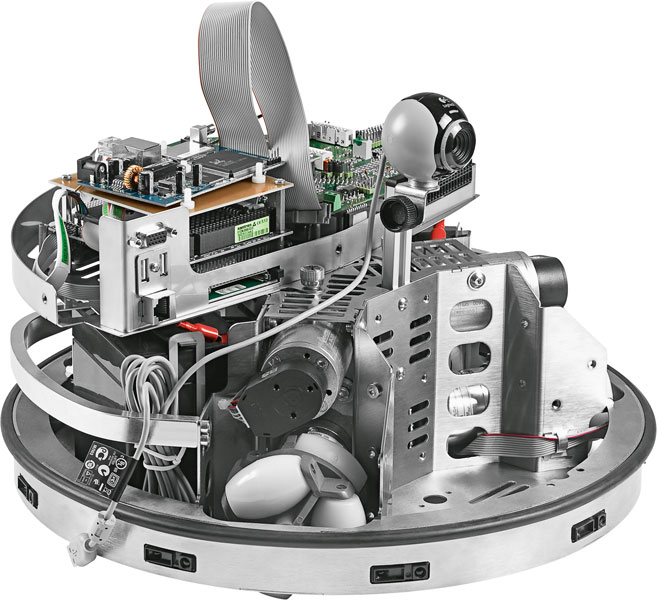
\includegraphics[width=.5\textwidth]{RobotinoOpen.jpg}
\label{apx:fig:robotinoopen}
\end{figure}


The controller housing is connected to the wiring in the chassis via
one plug-in. Thus you can easily take off the controller housing and
you have direct access to the mechanical system. The controller system
of Robotino® is divided into two parts – an embedded PC and a
microcontroller interface card: The Controller of Robotino® consists of
an embedded PC and a microcontroller interface board. The main
controller is the embedded PC 104 plus controller with the 500 MHz
processor AMD LX800. The PC has a SDRAM of 128 MB and is provided with
a 1 GB flash card. There are numerous communication interfaces on
board:

\begin{itemize}
\item 2 $\times$ 100 Mbit Ethernet
\item 2 $\times$ q external USB, 1 $\times$ on-board USB-connector
\item 2 $\times$  RS232
\item 1 $\times$ Parallel port and 1 $\times$ VGA port
\item Wireless LAN Access Point following the standards 802.11/b/g.
\item The access point can be switched into a client mode.  As an
  option you may use WPA2-coding.
\end{itemize}

\subsubsection{Software}
Preinstalled is an Ubuntu Linux operating system with real time kernel
running on the embedded PC 104. The main part of the controller is the
Robotino® server, a real time Linux application. It controls the drive
units and provides interfaces to communicate with external PC
applications via WiFi. There is an API with libraries which allow you
to create applications for Robotino® in numerous programming languages:

\begin{itemize}
	\item C++ und C 
	\item C\# 
	\item .net and JAVA 
	\item MatLab and Simulink
	\item Labview
\end{itemize}

You may find a lot of examples concerning using the different API’s in
the public forum “Openrobotino”, http://www.openrobotino.org .

\paragraph{Robotino® View} 

Robotino® View is a graphical programming language with numerous
prepared function blocks you can easily connect via input and output
parameters to establish more complicated function diagrams. You can use
these function diagrams as subprograms for more complex programming
sequences. To build up general programming sequences Robotino® View
follows the international standard IEC 61131-3. You may run Robotino®
View on an external PC and Robotino® View communicates directly with
the Robotino® Server on the PC 104 via WiFi in order to control the
robot system. The function blocks receive a direct feedback of the
hardware components such that you can live interact with the robot
system. On the other hand you can download Robotino® View programs into
the PC 104 in order to run the applications completely autonomously.
There is a well defined interface to develop own function blocks in C++
or Lua.

\paragraph{Image Processing}

Depending on the Robotino version it might happen that the standard web
camera only provides image data by jpeg compression. This is very
useful if you run your image processing on the PC and exchange the data
via WiFi. However, if you would like to run your image processing
algorithms on the Robotino controller then the processor is not
powerful enough in order to pack and to unpack the image data in a
reasonable time. Thus we recommend for running image processing
algorithms on the Robotino controller to use a camera without jpeg
compression, e.g. use the low cost Logitech web camera C250.

\subsection{Machines} \label{abx:sec:machine}

\begin{figure}[h]
	\centering
	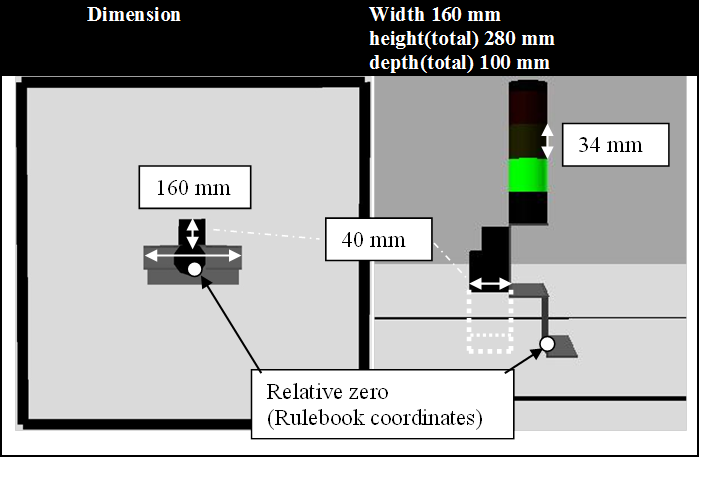
\includegraphics[width=.5\textwidth]{machine_measures.png}
	\caption{Ranges and dimensions of a signal}
	\label{apx:fig:machinemeasures}
\end{figure}

\subsubsection{Brackets}

\begin{figure}[h]
	\centering
	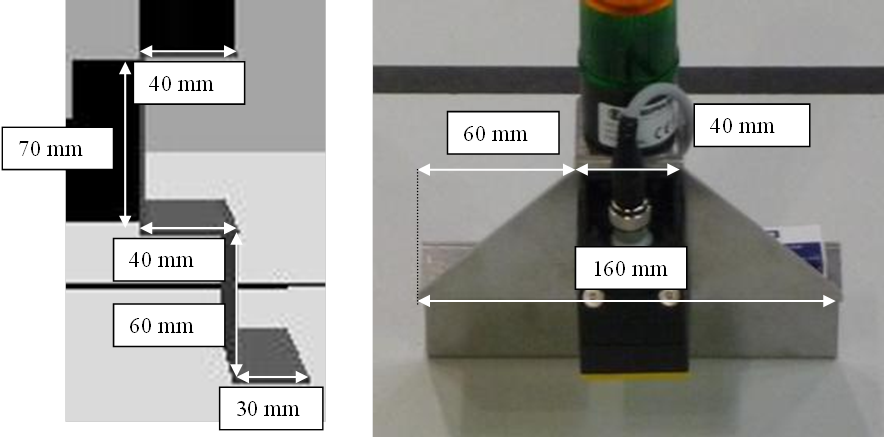
\includegraphics[width=.5\textwidth]{bracket.png}
	\caption{Ranges and dimensions of the supporting brackets}
	\label{apx:fig:brackets}
\end{figure}

\subsubsection{Signal}

\begin{table}[H]
  \centering
  \mytable{\begin{tabularx}{\linewidth}{l|X}
      \hline
      Dimension \&	diameter&	\SI{36}{\milli\metre} \\
      height(total)		 	&	\SI{147}{\milli\metre} \\
      Segment height 			&	\SI{34}{\milli\metre},
      including \SI{5}{\milli\metre} unlighted border \\
      Lifespan				&	max. \SI{50.000}{\hour} \\
      Connector				&	Bottom, \SI{2}{\metre} supplied 
      Compatible to the I/O-Terminal of MPS(r) units. \\
      Safety					&	IP65 \\
      Voltage					&	\SI{24}{\volt} \\
      Current					&	3 $\times$ \SI{40}{\milli\ampere} \\
      Kind of current			&	DC \\
      Operating mode			&	\SIrange{-20}{+50}{\degreeCelsius} \\
      Signaltype				&	Static LED \\
      Signal					&	Ultrabright LED\\
      Source					&	Festo \# 549843 \\
%      \hline
    \end{tabularx}}
  \caption{Technical specification of the signal}
  \label{apx:tab:signalproperties}
\end{table}

\subsubsection{RFID device}

\begin{table}[H]
  \centering
  \mytable{\begin{tabularx}{1\linewidth}{l|X}
      \hline
      Technical data of the read/write head		&	Housing rectangular \\
      Housing and working dimensions 				&
      \SI{40x40}{\milli\metre}  with the centred RFID
      tag. \\
      Housing height
      & \SI{65}{\milli\metre} \\ 
      Operating voltage							&	DC \\
      Housing material Plastic					& 	PBT-GF30-V0, black \\
      Material active face Plastic				& 	PA6-GF30, yellow \\
      Operating voltage
      & 	\SIrange{10}{30}{\volt.DC} \\
      DC rated operational current				& 	$\le$ \SI{80}{\milli\ampere} \\
      Data transfer								& 	inductance coupling \\
      Working frequency							& 	\SI{13.56}{\mega\hertz} \\
      Radio communication and protocol standards	&	ISO 15693 \\
      Read/write distance							&	max. \SI{115}{\milli\metre} \\
      Output function								&	4-wire, read/write \\
      Electrical connection 						&	Connectors M12 $\times$ 1 \\
       Vibration resistance						&	\SI{55}{\hertz} (\SI{1} {\milli\metre}) \\
       Shock resistance							&	\SI{30}{\gram} (\SI{11}{ \milli\second}) \\
       Protection class							&	IP67 \\
       Operating voltage display					& 	LED green \\
% %      \hline
    \end{tabularx}}
  \caption{Technical specification of the signal}
  \label{apx:tab:rfidproperties}
\end{table}

\subsubsection{Wifi equipment}
\label{sec:wifi-equipment}
\begin{table}[H]
  \centering
  \mytable{
    \begin{tabularx}{1\linewidth}{l|X}
      \hline
      Festo AP		&	LANCOM L-322agn \\
      Transfer rate		&	Up to \SI{108}{\mega\bit\per\second} \\
      Data link protocol	&	802.11 a/g/n \\
      Frequency			&	\SI{5.0}{\giga\hertz} \\
      IP-distribution		&	172.26.200.xxx for LAN clients(DHCP) \\
      &	172.26.101.xxx for the Robotino devices \\
      &	172.26.1.xxx for Robotinos \\
      Subnetmask			&	255.255.0.0 \\
      Encryption			&	Unsecured \\
      SSID				&	Separated for both teams:\\
      &	RobotinoEvent.1 \\
      & RobotinoEvent.2 \\
      Festo Clients		&	3COM WL-560 \\
      Power Supply		&	Clients: \SI{12}{\volt}, \SI{1}{\ampere},\\
      & 	Most Laptops cannot power them \\
      & 	via USB! \\
      Connector			&	Ethernet \\
      
%      \hline
    \end{tabularx} }
    \caption{Technical specification of the signal}
	\label{apx:tab:wifi}
\end{table}

\subsubsection{Data carrier}
\begin{table}[H]
  \centering
  \mytable{
    \begin{tabularx}{\linewidth}{l|X}
      \hline
      Dimension									&	\diameter  \SI{20}{\milli\metre} \\
      Height										&	\SI{2.5}{\milli\metre} \\
      Data transfer								&	inductance coupling \\
      Working frequency							&	\SI{13.56}{\mega\hertz} \\
      Memory 										&	read/write \\	
      Memory type									&	EEPROM \\
      Memory size									&	\SI{128}{\byte} \\
      Freely usable memory						&	\SI{112}{\byte} \\
      Number of read operations					&	unlimited \\
      Number of write operations					&	105 \\
      Typical read time							&	\SI{2}{\milli\second\per\byte} \\
      Typical write time							&	\SI{3}{\milli\second\per\byte} \\
      Radio communication and protocol standards	&	ISO 15693 \\
      
      % \hline
    \end{tabularx}}
  \caption{Technical specification of the signal}
  \label{apx:tab:datacarrier}
\end{table}


\end{appendix}
\end{document}
